\chapter{State Space Analysis}

In order to use the generated .cpn file for state space analysis, preliminary knowledge on (1) the concept of colored petri nets, and (2) the concepts of the CPN Tools 4 Tool Suite. 

Open CPN\_Analysis\_Model.cpn using CPN Tools 4. The Analysis\_Model canvas in the model should look like this:

\begin{figure}[ht]
\centering
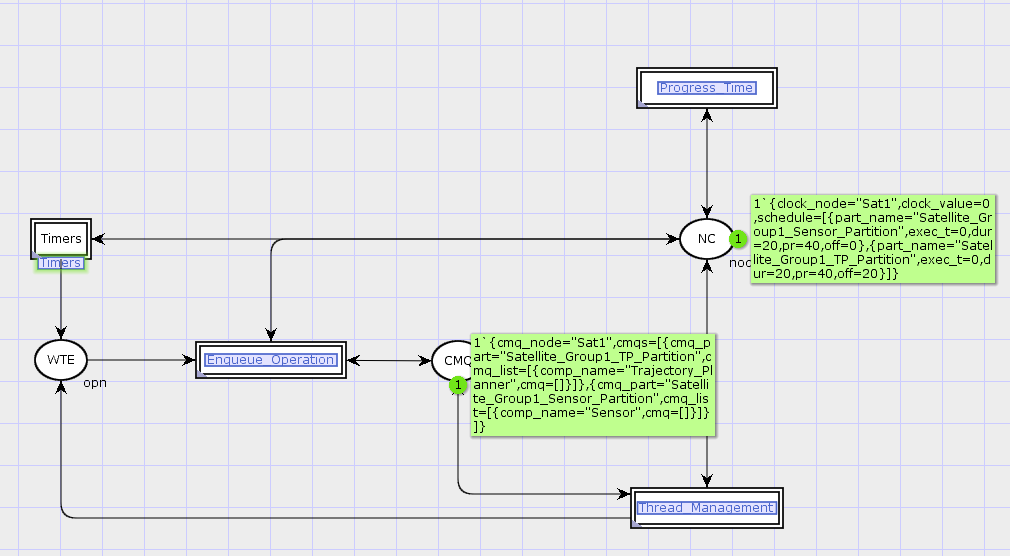
\includegraphics[width=0.9\textwidth]{./figs/Analysis}
\caption{CPN Analysis Model}
\label{fig:analysis}
\vspace{-0.2in}
\end{figure}
\vspace{0.1in} 

The colored petri net tokens in this model are application-specific and created by CPNGenerator when it parses the application. Now drag the State Space Tool onto the canvas. The settings on the state space tool can be set by right clicking on \emph{SS} tool and clicking on \emph{Set Options}. For the trajectory planner application, set the settings as shown in Figure \ref{fig:sss}.

Use the state space tool to generate a bounded state space for the analysis model using the applied settings. A successful bounded state space generation leads to a prompt as shown in Figure \ref{fig:sss}.

Once a bounded state space is generated, it is time to search this state space and obtain useful analysis results. The page Analysis\_Model consists of a set of state space queries generated by CPNGenerator. Use the \emph{ML!} tool (ML evaluate) to evaluate standard ML code (the state space queries).

\begin{figure}[ht]
\centering
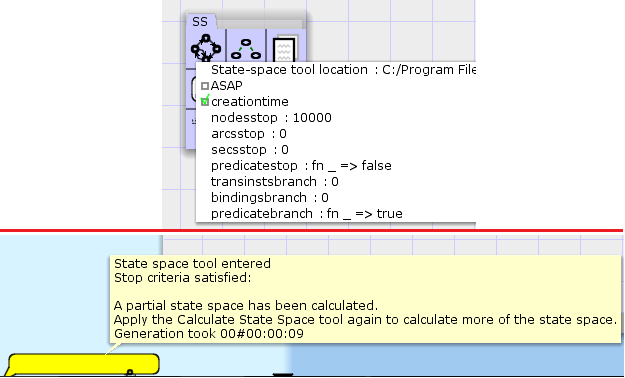
\includegraphics[width=0.9\textwidth]{./figs/SSS}
\caption{State Space Tool}
\label{fig:sss}
\vspace{-0.2in}
\end{figure}
\vspace{0.1in} 

\subsection{Deadline Violation Detection}
Using the \emph{op\_st} and \emph{op\_et} fields of every component operation, the model is capable of identifying deadline violations in component operations that are either currently in progress or waiting in the component message queue. The model essentially takes a snapshot of such cases and records the time stamps. For instance: In Figure \ref{fig:tpa_td}, the \emph{on\_one\_data} on the Trajectory Planner Component starts at time = 20 and completes at time = 76, taking 56 ms accounting for temporal partitioning and the block time due to the remote call. If the deadline for this operation were to be set at 50 ms, the model would take notice of the violation at time = 51. This can also be observed by relying on the simulation tool as there is only one thread execution order for this scenario. Figures \ref{fig:cpn_tpa_dv_marking} and \ref{fig:cpn_tpa_dv_ss} show the observed deadline violation and the state space queries that reinforce the observation. The \emph{SearchNodes} function enables searching parts of the state space and identifying nodes that support a predicate function. In this case, the predicate function obtains state space nodes where a deadline violation is recorded in the \emph{Late\_Op} place. From this subset of nodes, unique deadline violations are identified. A backtrace for the observed violation can be easily obtained by using the \emph{NodesInPath (InitialNode, DestNode)} function that presents an ordered list of state space nodes from the initial node that represents the path taken to reach the violation node.

\begin{figure}[ht]
\centering
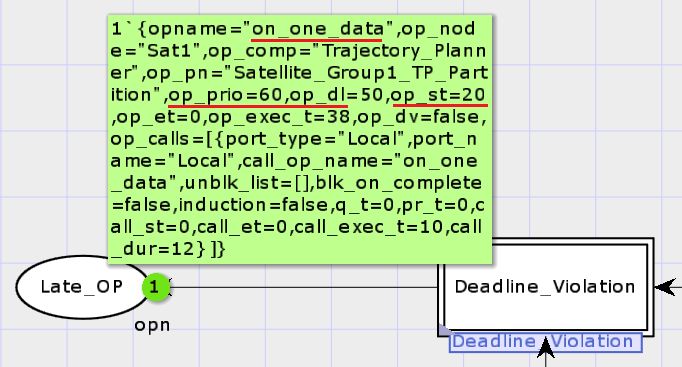
\includegraphics[width=0.60\textwidth]{./figs/cpn_tpa_dv_marking}
\caption{Observed Deadline Violation}
\label{fig:cpn_tpa_dv_marking}
\vspace{-0.2in}
\end{figure}
\vspace{0.1in}

\begin{figure}[ht]
\centering
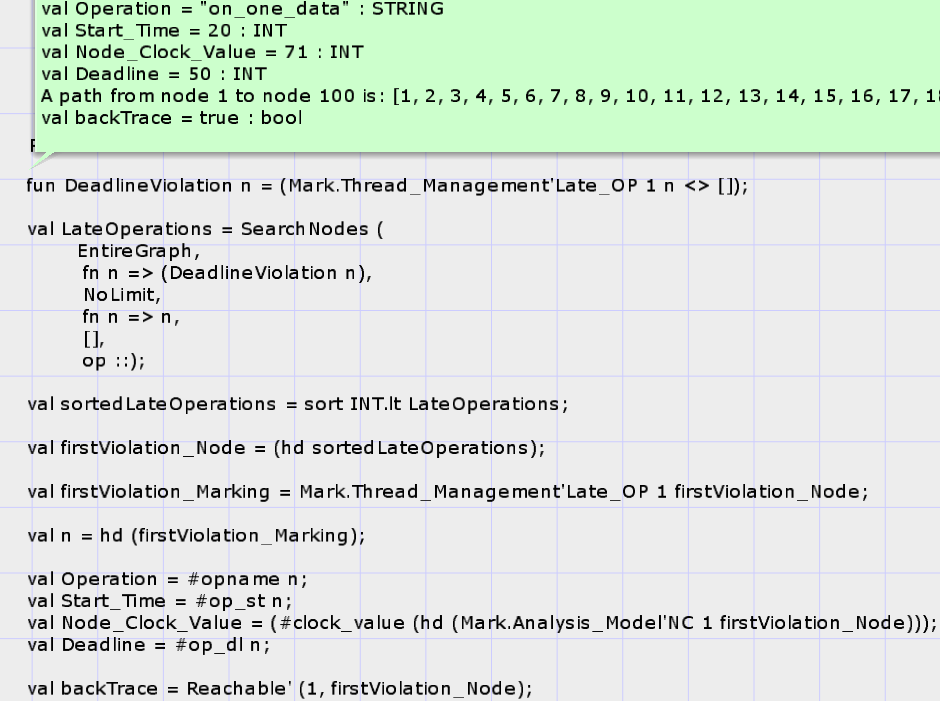
\includegraphics[width=0.99\textwidth]{./figs/cpn_tpa_dv_ss}
\caption{State Space Query for Deadline Violation Detection}
\label{fig:cpn_tpa_dv_ss}
\vspace{-0.2in}
\end{figure}

\subsection{Worst-case Trigger-to-Response Time Calculation}

As component operations run to completion, the analysis model keeps track of operation completion using a \emph{COP} place as shown in Figure \ref{fig:cpn_completed_operations}. 

\begin{figure}[ht]
\centering
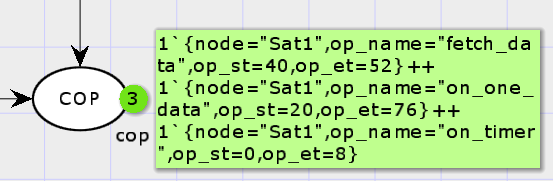
\includegraphics[width=0.60\textwidth]{./figs/cpn_completed_operations}
\caption{Completed Operations}
\label{fig:cpn_completed_operations}
\vspace{-0.2in}
\end{figure}
\vspace{0.1in}

For a known trigger operation and desired response operation, the worst-case trigger-to-response time can also be calculated from the generated state space. This is especially useful when multiple threads of same priority share a partition leading to a tree of possible thread execution orders. Once the necessary partial state space is generated, by using the operation IDs of the trigger and response, the earliest completion of the trigger operation and the latest completion of the response operation within the set period are identified. In the Trajectory Planning application, considering the \emph{on\_timer} to be the trigger and the trajectory planning \emph{on\_one\_data} to be the response, the worst-case response time is found to be 65 ms as shown in Figure \ref{fig:cpn_tpa_trigger_response_time}. Since all of the necessary information is already packed in the state space, variants of such queries can be easily constructed without changing the model.

\begin{figure}[ht]
\centering
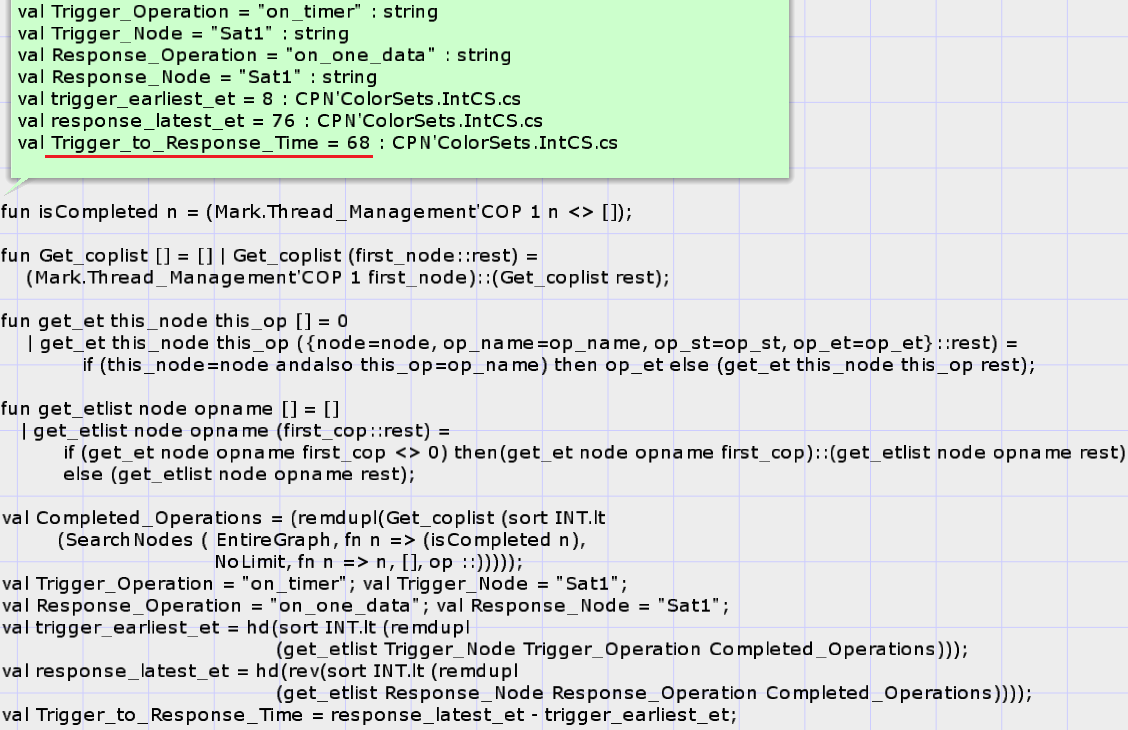
\includegraphics[width=0.99\textwidth]{./figs/cpn_tpa_trigger_response_time}
\caption{Worst-Case Trigger-to-Response Time Calculation}
\label{fig:cpn_tpa_trigger_response_time}
\vspace{-0.2in}
\end{figure}
\vspace{0.1in}

It must be noted here that understanding the state space queries requires knowledge on standard ML code. Using standard ML, similar queries can be written as auxillary text in the CPN page. 
